\subsection{view}
\label{subsec:view}

Das view Package enthält alle Klassen, die für die Graphische Benutzeroberfläche vonnöten sind. UI Elemente wie Menüs, Buttons, Toolbars und im Allgemeinen das Layout werden durch die Javafx internen \glspl{fxml-datei} beschrieben. Aus diesem Grund ist der eigentliche Aufbau davon nicht modelliert.
Jeder View ist durch einen ViewController vertreten. Im Controller können Commands auf die jeweiligen Interactions eines Views gemappt werden. Da ein View das INotifier Interface implementiert, kann er diese Interactions durch bestimmte Benutzeraktionen ausführen. Daraufhin wird der jeweilig gemappte Command zum Listener geschickt.
Der NetworkGraphView in \gls{programname} implementiert das VisualizationServer Interface aus der JUNG Bibliothek. Dies ermöglicht es kompatibel zu den Funktionen der Bibliothek zu bleiben und dennoch in die JavaFX Struktur eingebunden zu werden.

\clearpage
\begin{sidewaysfigure}
  \centering
  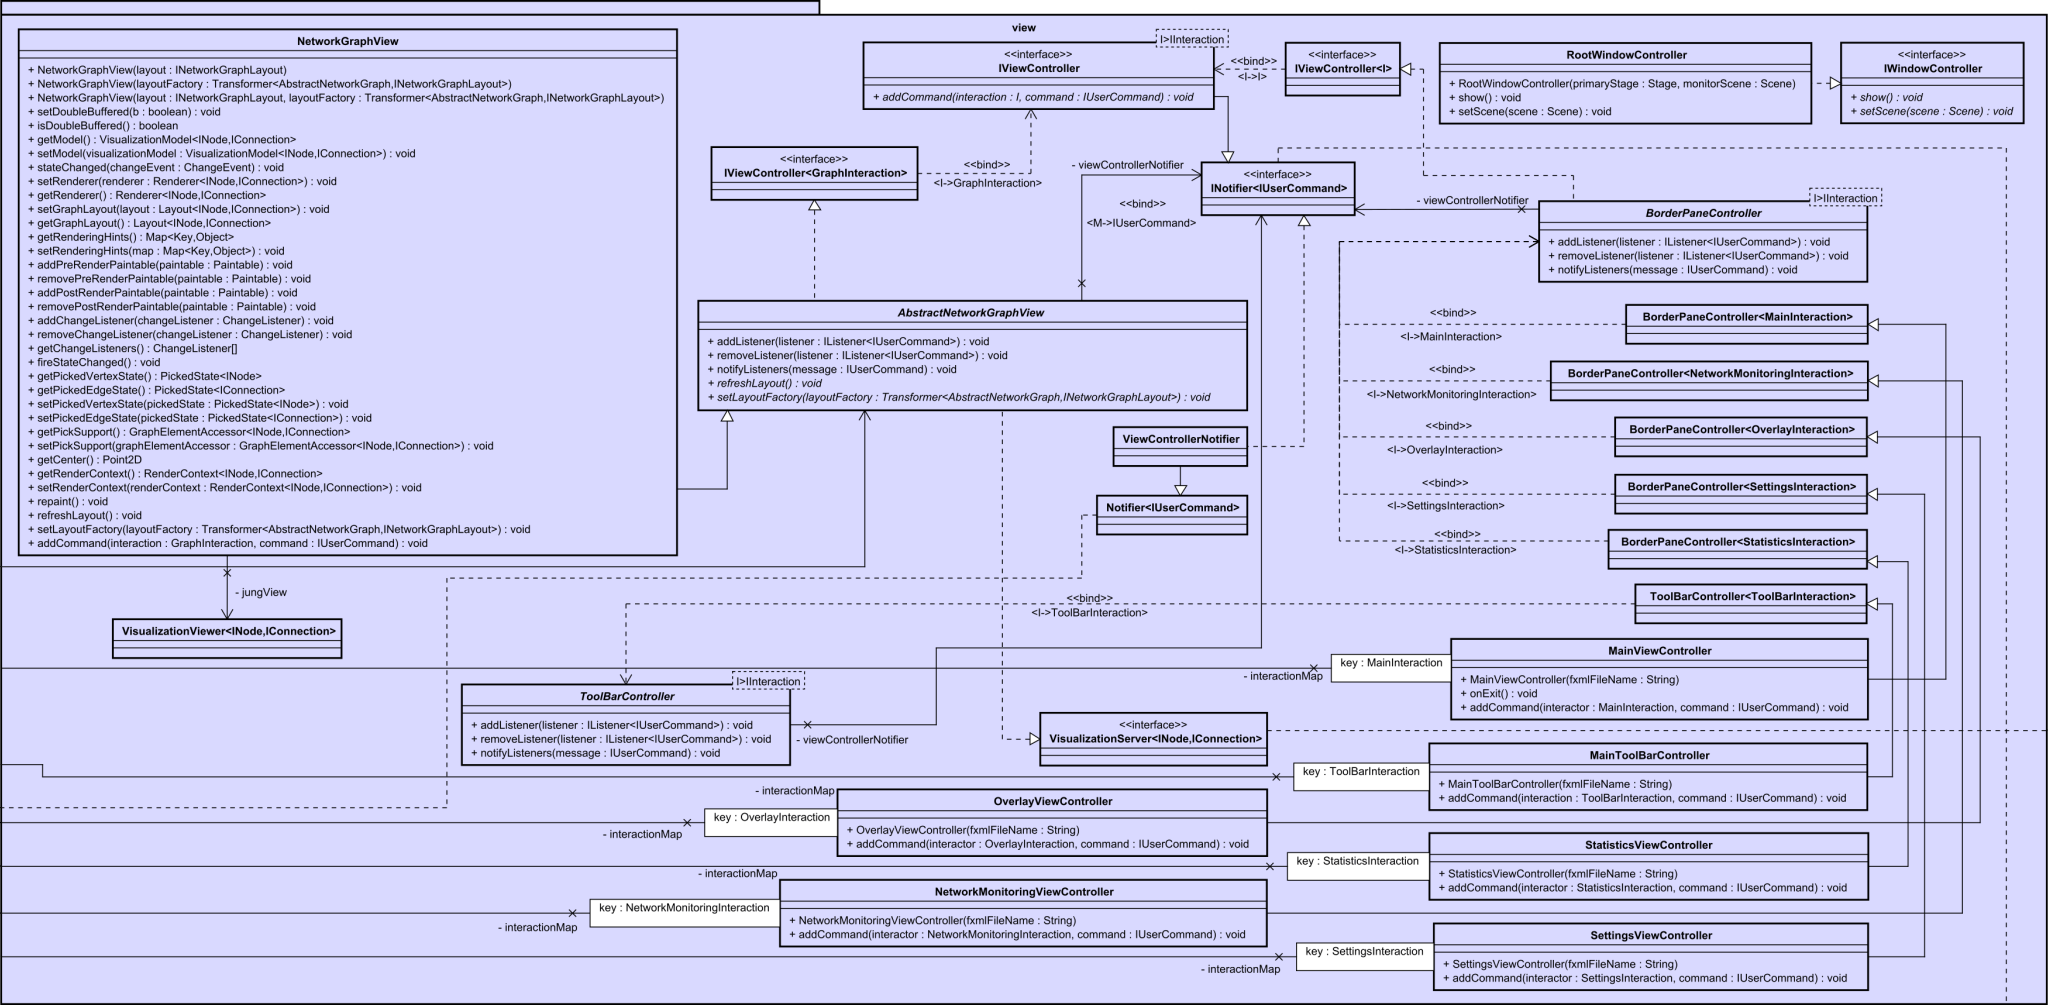
\includegraphics[width=\textwidth]{../diagramimages/view.png}
  \caption{replaylogging-Package}
\end{sidewaysfigure}
\clearpage
